
\حصہ{بنیادی نقش اور دیگر نمونی استعمال}
اس باب میں ریمان مجموعہ کے استعمال سے ہم نے چیزوں کا حساب کرنا سیکھا۔ یہ عمل درج ذیل تین اقدام پر مشتمل ہے۔
\begin{enumerate}[a.]
\item
مطلوبہ چیز کو ایک یا ایک سے زائد تفاعل سے ظاہر کیا جاتا ہے جو بند وقفہ \عددی{[a,b]} پر استمراری ہوں۔
\item
وقفہ \عددی{[a,b]} کی خانہ بندی کر کے ہر ذیلی وقفہ میں ایک نقطہ \عددی{c_k} منتخب کیا جاتا ہے۔ \عددی{k} ویں ذیلی وقفہ کی لمبائی \عددی{\Delta x_k}  ہو گی۔ 

مطلوبہ چیز کی تخمینی قیمت کو مجموعہ کی صورت میں لکھا جاتا ہے۔

اس مجموعہ کی شناخت بطور وقفہ \عددی{[a,b]} پر استمراری تفاعل کی ریمان مجموعہ کی جاتی ہے۔
\item
خانہ بندی کا معیار صفر کے قریب تر کرنے سے ریمان مجموعہ بہتر سے بہتر نتیجہ دے گا۔

ریمان مجموعہ کا حد قطعی تکمل ہو گا۔

قطعی تکمل استعمال کرتے ہوئے چیز کا حساب لگایا جاتا ہے۔
\end{enumerate}

درج بالا اقدام سے لکیر کی لمبائی، خطے کا رقبہ، اجسام کا حجم، کام، وغیرہ کا حساب ممکن ہے۔

حقیقت میں انجینئری، حیاتیات، علم کیمیا، اقتصادیات، ارضیات، طب، اور دیگر شعبوں میں ہزاروں کی تعداد میں چیزوں کو ان اقدام سے حل کیا جا سکتا ہے۔

اس حصہ میں ان اقدام پر دوبارہ غور کیا جائے گا اور کئی نئے تکمل متعارف کیے جائیں گے جو ان اقدام سے پیدا ہوتے ہیں۔

\جزوحصہء{فاصلہ بالمقابل ہٹاو}
اگر کسی محددی لکیر پر ایک جسم کا مقام تفاعل \عددی{s(t)} دیتا ہو اور یہ جسم ایک ہی سمت میں حرکت کرتا ہو تب   \عددی{t=a} سے \عددی{t=b} تک جسم کے سمتی رفتار تفاعل \عددی{v(t)} کا تکمل  اس دورانیے میں طے شدہ فاصلہ دے گا۔ اگر جسم اس دورانیے میں سمت تبدیل کرتا ہو تب طے شدہ فاصل حاصل کرنے کے لئے ہمیں جسم کی رفتار \عددی{\abs{v(t)}} کا تکمل لینا ہو گا۔ جسم کی سمتی رفتار کا تکمل جسم کا \اصطلاح{ہٹاو}\فرہنگ{ہٹاو}\حاشیہب{displacement}\فرہنگ{displacement} \عددی{s(b)-s(a)} دے گا جو اس کی ابتدائی اور اختتامی مقامات کے بیچ فاصلہ ہے۔

یہ دیکھنے کے لئے ہم وقتی وقفہ \عددی{a\le t\le b} کی خانہ بندی کرتے ہیں جہاں \عددی{k} ویں وقفے کی لمبائی  \عددی{\Delta t_k} ہے۔ اگر \عددی{\Delta t_k} بہت کم ہو تب دورانیہ \عددی{t_{k-1}} تا \عددی{t_k} جسم کی سمتی رفتار \عددی{v(t)} میں تبدیلی قابل نظر انداز ہو گی لہٰذا اس ذیلی وقفے کی دائیں سر پر جسم کی سمتی رفتار \عددی{v(t_k)} کو اس ذیلی وقفہ پر جسم کی سمتی رفتار تصور کیا جا سکتا ہے۔ یوں \عددی{k} ویں ذیلی وقفہ کے دوران جسم کے مقام میں تبدیلی درج ذیل ہو گی۔
\begin{align*}
v(t_k)\Delta t_k
\end{align*}
اگر \عددی{v(t_k)} مثبت ہو تب یہ تبدیلی مثبت ہو گی اور اگر \عددی{v(t_k)} منفی ہو تب یہ تبدیلی منفی ہو گی۔ دونوں صورتوں میں \عددی{k} ویں ذیلی وقفہ میں جسم 
\begin{align*}
\abs{v(t_k)}\Delta t_k
\end{align*}
فاصلہ طے کرے گا۔یوں پورے وقفے پر جس کل درج ذیل فاصلہ طے کرے گا۔
\begin{align}\label{مساوات_تکمل_استعمال_طے_فاصلہ}
\sum_{k=1}^n \abs{v(t_k)}\Delta t_k
\end{align}
مساوات \حوالہ{مساوات_تکمل_استعمال_طے_فاصلہ} میں مجموعہ، وقفہ \عددی{[a,b]} پر تفاعل رفتار  \عددی{\abs{v(t)}} کا ریمان مجموعہ ہے۔ ہم توقع کرتے ہیں کہ خانہ بندی کا معیار صفر کے قریب تر کرنے سے یہ تخمینی مجموعہ  بہتر نتیجہ دے گا۔ یوں ایسا معلوم ہوتا ہے کہ وقفہ \عددی{[a,b]} میں جسم کا طے شدہ فاصلہ حاصل کرنے کے لئے درج ذیل تکمل استعمال کیا جا سکتا ہے۔
\begin{align}
\text{\RL{طے شدہ فاصلہ}}=\int_a^b \abs{v(t)}\dif t
\end{align}
یہ ریاضیاتی نمونہ ہر بار بالکل درست فاصلہ دیتا ہے۔

اگر ہم جاننا چاہتے ہیں کہ وقتی دورانیے کی اختتام پر  ابتدائی مقام سے جسم کتنا دور ہو گا تب ہم \عددی{v(t)} کا تکمل  نا کہ \عددی{\abs{v(t)}} کا تکمل لیں گے۔

آئیں دیکھیں ایسا کیوں ہو گا۔ فرض کریں کی تفاعل \عددی{s(t)}جسم کا مقام دیتا ہے اور \عددی{F} تفاعل \عددی{v} کا الٹ تفرق ہے۔ تب
\begin{align*}
s(t)=F(t)+C
\end{align*}
ہو گا جہاں \عددی{C} مستقل ہے۔ یوں لمحہ \عددی{t=a} سے \عددی{t=b} تک جسم کا ہٹاو 
\begin{align*}
s(b)-s(a)=(F(b)+C)-(F(a)+C)=F(b)-F(a)=\int_a^bv(t)\dif t
\end{align*}
ہو گا یعنی:
\begin{align}
\text{ہٹاو}=\int_a^bv(t)\dif t
\end{align}

\ابتدا{مثال}\شناخت{مثال_تکمل_استعمال_فاصلہ_ہٹاو}
ایک لکیر پر لمحہ \عددی{t=0} سے لمحہ \عددی{t=\tfrac{3\pi}{2}\,\si{\second}} تک  ایک جسم کی رفتار \عددی{v(t)=5\cos t\,\si{\meter\per\second}} ہے۔ یہ جسم کل کتنا فاصلہ طے کرتا ہے؟ اس کا کل ہٹاو کتنا ہو گا؟

حل:\quad
\begin{align*}
\text{\RL{طے شدہ فاصلہ}}&=\int_0^{\tfrac{3\pi}{2}}\abs{5\cos t}\dif t&&\text{\RL{رفتار لا تکمل فاصلہ ہو گا}}\\
&=\int_0^{\tfrac{\pi}{2}} 5\cos t \dif t+\int_{\tfrac{\pi}{2}}^{\tfrac{3\pi}{2}}(-5\cos t)\dif t\\
&=\left. 5\sin t\right]_0^{\tfrac{\pi}{2}}\left.-5\sin t\right]_{\tfrac{\pi}{2}}^{\tfrac{3\pi}{2}}\\
&=5(1-0)-5(-1-1)=5+10=\SI{15}{\meter}
\end{align*}
\begin{align*}
\text{ہٹاو}&=\int_0^{\tfrac{3\pi}{2}}5\cos t\dif t&&\text{\RL{سمتی رفتار کا تکمل ہٹاو ہو گا}}\\\
&=\left.5\sin t\right]_0^{\tfrac{3\pi}{2}}=5(-1)-5(0)=\SI{-5}{\meter}
\end{align*}
اس دورانیے میں جسم \عددی{\SI{5}{\meter}} آگے اور \عددی{\SI{10}{\meter}} پیچھے سفر کرتا ہے۔ یوں یہ \عددی{\SI{15}{\meter}} فاصل طے کرتا ہے جبکہ اس کا ہٹاو \عددی{\SI{-5}{\meter}} ہو گا (شکل \حوالہ{شکل_مثال_تکمل_استعمال_فاصلہ_ہٹاو})۔
\انتہا{مثال}
%=========================
\begin{figure}
\centering
\begin{subfigure}{0.45\textwidth}
\centering
\begin{tikzpicture}
\pgfmathsetmacro{\ka}{1/2*pi}
\pgfmathsetmacro{\kb}{pi}
\pgfmathsetmacro{\kc}{3/2*pi}
\begin{axis}[small,axis lines=middle,xlabel={$t\,[\si{\second}]$},ylabel={$v\,[\si{\meter\per\second}]$},enlargelimits=true,xlabel style={at={(current axis.right of origin)},anchor=west},ylabel style={at={(current axis.above origin)},anchor=south},xtick={\ka,\kb,\kc},xticklabels={$\tfrac{\pi}{2}$,$\pi$,$\tfrac{3\pi}{2}$},ytick={-5,5}]
\addplot[domain=0:3*pi/2]{5*cos(deg(x))};
\end{axis}
\end{tikzpicture}
\caption{سمتی رفتار تفاعل۔}
\end{subfigure}\hfill
\begin{subfigure}{0.45\textwidth}
\centering
\begin{tikzpicture}
\pgfmathsetmacro{\ka}{1/2*pi}
\pgfmathsetmacro{\kb}{pi}
\pgfmathsetmacro{\kc}{3/2*pi}
\begin{axis}[small,axis lines=middle,xlabel={$t\,[\si{\second}]$},ylabel={$s\,[\si{\meter}]$},enlargelimits=true,xlabel style={at={(current axis.right of origin)},anchor=west},ylabel style={at={(current axis.above origin)},anchor=south},xtick={\ka,\kb,\kc},xticklabels={$\tfrac{\pi}{2}$,$\pi$,$\tfrac{3\pi}{2}$},ytick={-5,5}]
\addplot[domain=0:3*pi/2]{5*sin(deg(x))};
\end{axis}
\end{tikzpicture}
\caption{ابتدائی نقطہ $s(0)$ سے جسم کا ہٹاو۔}
\end{subfigure}
\caption{سمتی رفتار تفاعل اور ہٹاو (مثال \حوالہ{مثال_تکمل_استعمال_فاصلہ_ہٹاو})}
\label{شکل_مثال_تکمل_استعمال_فاصلہ_ہٹاو}
\end{figure}

\جزوحصہء{قاعدہ دولس}
آپ جانتے ہیں کہ  چننے کے بعد سیب کا ذائقہ  وقت کے ساتھ تبدیل ہوتا ہے۔ سیب میں شکر وقت کے ساتھ نشاستہ میں تبدیل ہوتا ہے۔ سیب میں نشاستہ کی مقدار معلوم کرنے کے لئے ہم سیب کا ایک باریک کتلے  کو خوردبین میں دیکھتے ہیں۔ نشاستہ کے ہر دانہ کا سطح عمودی تراش خوردبین میں صاف نظر آتا ہے لہٰذا کتلے کی سطح میں نشاستہ کے رقبہ عمودی تراش کا تناسب معلوم کیا جا سکتا ہے۔ یہ دو بعدی تناسب سیب میں نشاستہ کے تین بعدی تناسب کے برابر ہو گا۔ دو بعدی اور تین بعدی تناسب کی یکسانیت  اوسط قیمت کی تصور پر مبنی ہے۔

فرض کریں ہم کسی ٹھوس  جسم میں دانہ دار مادہ کی تناسب جاننا چاہتے ہیں۔ ہم ٹھوس جسم سے موزوں نمونہ حاصل کرتے ہیں جس کو کاٹ کر ایک مکعب حاصل کیا جاتا ہے۔ اس مکعب کا ضلع \عددی{L} ہے۔ اس مکعب کو شکل \حوالہ{شکل_تکمل_استعمال_مسئلہ_دوسل} میں دکھایا گیا ہے جہاں مکعب کا ضلع \عددی{x} محور پر  ہے۔ ہم وقفہ \عددی{[0,L]} کے عمودی سطحوں سے اس مکعب کو کتلوں میں تقسیم کرتے ہیں۔ فرض کریں \عددی{x} پر دانہ دار مادے کے رقبے کا تناسب \عددی{r(x)} ہے۔ فرض کریں کہ \عددی{r(x)} متغیر \عددی{x} کا استمراری تفاعل ہے۔ 

اب وقفہ \عددی{[0,L]} کی خانہ بندی کریں۔نقطہ خانہ بندی پر \عددی{x} محور کے عمودی سطحوں سے مکعب کو کتلوں میں تقسیم کریں۔ \عددی{k} ویں ذیلی وقفے کی لمبائی \عددی{\Delta x_k} ہو گی جو نقطہ \عددی{x_{k-1}} اور نقطہ \عددی{x_k} پر موجود سطحوں کے بیچ فاصلہ ہو ہے۔اگر یہ سطحیں کافی قریب ہوں تب یہ دانوں کو بیلنی شکل میں کاٹیں گے۔ ان بیلنوں کا قاعدہ \عددی{x_k} پر ہو گا۔ ان سطحوں کے بیچ دانہ دار مادہ کی حجمی تناسب وہی ہو گی جو \عددی{x_k} پر سطح میں دانہ دار مادہ کی سطحی تناسب ہے جو ان بیلنوں کے قاعدہ کے برابر ہے جو از خود تقریباً \عددی{r(x)} ہو گا۔یوں دو قریبی سطحوں کے بیچ دانہ دار مادہ کی مقدار درج ذیل ہو گی۔
\begin{align*}
(\text{\RL{تناسب}})\times(\text{\RL{کتلے کا حجم}})=r(x)L^2\Delta x_k
\end{align*}

پورے مکعب میں دانہ دار مادہ کی مقدار
\begin{align*}
\sum_{k=1}^nr(x)L^2\Delta x_k
\end{align*}
ہو گی جو وقفہ \عددی{[0,L]} پر تفاعل \عددی{r(x)L^2} کا ریمان مجموعہ ہے۔ ہم توقع کرتے ہیں کہ خانہ بندی کا معیار صفر کے قریب پہنچانے سے یہ مجموعہ بہتر سے بہتر نتیجہ دے گا لہٰذا درج ذیل تکمل، جو ریمان مجموعہ کی حد کو ظاہر کرتا ہے، مکعب  میں دانہ دار مادہ کی مقدار دے گا۔
\begin{align*}
\int_0^L r(x)L^2\dif x
\end{align*}

اس مقدار کو مکعب کے حجم \عددی{L^3} سے تقسیم کرنے سے مکعب میں دانہ دار مادہ کی تناسب حاصل ہو گی۔ اگر ہم نے موزوں نمونی مکعب منتخب کیا ہو تب پورے ٹھوس جس میں دانہ دار مادہ کا تناسب وہی ہو گا جو اس نمونی مکعب میں ہے۔یوں درج ذیل ہو گا۔
\begin{align*}
\text{\RL{ٹھوس جسم میں دانہ دار مادہ کا تناسب}}&=\text{\RL{مکعب میں دانہ دار مادہ کا تناسب}}\\
&=\frac{\int_0^L r(x)L^2\dif x}{L^3}\\
&=\frac{1}{L}\int_0^L r(x)\dif x\\
&\text{\RL{نمائندہ سطح عمودی تراش میں دانہ دار مادے کا سطحی تناسب}}
\end{align*}
یہ \اصطلاح{قاعدہ دولس}\فرہنگ{قاعدہ!دولس}\حاشیہب{Delesse's rule}\فرہنگ{rule!Delesse's} ہے جسے فرانسیسی  ماہر ارضیات اشیلہ ارنسٹ دولس\عددی{ [1817-1881]} نے دریافت کیا۔ یوں وقفہ \عددی{[0,L]} پر \عددی{r(x)} کی اوسط قیمت \عددی{\bar{r}} سے ٹھوس جسم میں دانہ دار مادے کا تناسب حاصل ہو گا۔حقیقت میں کئی رقبہ عمودی تراش پر \عددی{\bar{r}} حاصل کر کے ان کی اوسط لی جاتی ہے۔ 

جناب دولس پتھر میں دانہ دار مادہ کی تناسب میں دلچسپی رکھتے تھے۔ وہ نمونی پتھر کی ایک سطح کو اچھی طرح چمکدار بنا کر سطح کے برابر مومی کاغذ کو چمکیلی سطح پر رکھ کر دانہ دار خطوں کی نشاندہی کرتے۔کاغذ کا وزن کرنے کے بعد، دانہ دار خطوں کو کاغذ سے کاٹ کر کاغذ کا وزن دوبارہ کرتے۔ یوں دانہ دار خطوں کے رقبہ کا تناسب حاصل کیا جاتا۔ یہ ترکیب آج بھی تیل کی تلاش میں استعمال کیا جاتا ہے۔
\begin{figure}
\centering
\begin{subfigure}{0.3\textwidth}
\centering
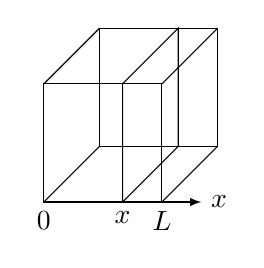
\begin{tikzpicture}
\pgfmathsetmacro{\d}{1}
\pgfmathsetmacro{\l}{1.5}
\pgfmathsetmacro{\ang}{45}
\draw(0,0)rectangle ++(\l,\l);
\draw(\ang:\d) rectangle ++(\l,\l);
\draw(2/3*\l,0)node[below]{$x$}--++(\ang:\d)--++(0,\l)--++(\ang:-\d)--++(0,-\l);
\draw(0,0)node[below]{$0$}--++(\ang:\d);
\draw(\l,0)node[below]{$L$}--++(\ang:\d);
\draw(0,\l)--++(\ang:\d);
\draw(\l,\l)--++(\ang:\d);
\draw[-latex](\l,0)--++(0.5,0)node[right]{$x$};
\end{tikzpicture}
\caption{}
\end{subfigure}\hfill
\begin{subfigure}{0.3\textwidth}
\centering
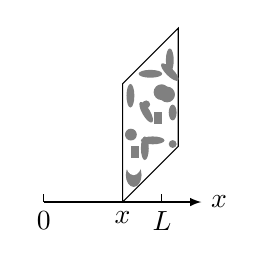
\begin{tikzpicture}
\pgfmathsetmacro{\d}{1}
\pgfmathsetmacro{\l}{1.5}
\pgfmathsetmacro{\ang}{45}
\draw(0,0)node[below]{$x$}--++(\ang:\d)--++(0,\l)--++(\ang:-\d)--++(0,-\l);
\draw[-latex](-2/3*\l,0)--++(\l+0.5,0)node[right]{$x$};
\draw(-2/3*\l,0)node[below]{$0$}--++(0,0.1)  (-2/3*\l+\l,0)node[below]{$L$}--++(0,0.1);
\fill[gray](\ang:0.2)++(0,0.2) circle (0.1cm and 0.15 cm);
\fill[white](\ang:0.2)++(0,0.35) circle (0.1cm and 0.15 cm);
\fill[gray](\ang:0.4)++(0,0.4) circle (0.05cm and 0.15 cm);
\fill[gray](\ang:0.4)++(0.1,0.5) circle (0.15cm and 0.05 cm);
\fill[gray](\ang:0.15)++(0,0.45) rectangle ++(0.1,0.15);
\fill[gray](\ang:0.56)++(0,0.6) rectangle ++(0.1,0.15);
\begin{scope}[shift={(0.2*\l,0.76*\l)}]
\fill[gray,rotate=30](0,0) circle (0.05cm and 0.15 cm);
\fill[gray](0,0.1) circle (0.05);
\end{scope}
\fill[gray](\ang:0.8)++(0,0.8) circle (0.1);
\fill[gray](\ang:0.7)++(0,0.9) circle (0.1);
\fill[gray](\ang:0.5*\d)++(0,0.85*\l)coordinate[](ka) circle (0.15cm and 0.05 cm);
\fill[gray,rotate around={45:(0.6*\d,1.1*\l)}](0.6*\d,1.1*\l)circle (0.05 cm and 0.15 cm);
\fill[gray,rotate around={0:(0.6*\d,1.2*\l)}](0.6*\d,1.2*\l)circle (0.05 cm and 0.15 cm);
\fill[gray,rotate around={0:(0.1*\d,0.9*\l)}](0.1*\d,0.9*\l)circle (0.05 cm and 0.15 cm);
\fill[gray](\ang:0.9*\d)++(0,0.1)circle (0.05 cm);
\fill[gray](\ang:0.15*\d)++(0,0.5*\l)circle (0.075 cm);
\fill[gray](\ang:0.9*\d)++(0,0.5)circle (0.05 cm and 0.1 cm);
\end{tikzpicture}
\caption{}
\end{subfigure}\hfill
\begin{subfigure}{0.3\textwidth}
\centering
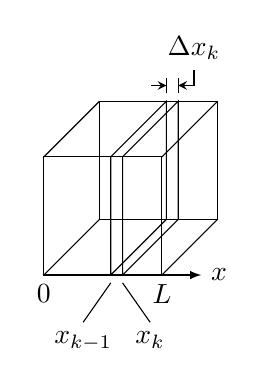
\begin{tikzpicture}
\pgfmathsetmacro{\d}{1}
\pgfmathsetmacro{\l}{1.5}
\pgfmathsetmacro{\ang}{45}
\draw(0,0)rectangle ++(\l,\l);
\draw(\ang:\d) rectangle ++(\l,\l);
\draw(2/3*\l-1/10*\l,0)--++(\ang:\d)--++(0,\l)--++(\ang:-\d)--++(0,-\l);
\draw(2/3*\l,0)--++(\ang:\d)--++(0,\l)--++(\ang:-\d)--++(0,-\l);
\draw(2/3*\l-1/10*\l,-0.1)--++(-0.35,-0.5)node[below]{$x_{k-1}$};
\draw(2/3*\l,-0.1)--++(0.35,-0.5)node[below]{$x_{k}$};
\draw(2/3*\l,\l)++(\ang:\d)++(0,0.1)--++(0,0.2)coordinate[pos=0.5](kR);
\draw(2/3*\l-1/10*\l,\l)++(\ang:\d)++(0,0.1)--++(0,0.2)coordinate[pos=0.5](kL);
\draw[stealth-](kR)--++(0.2,0)--++(0,0.2)node[above]{$\Delta x_k$};
\draw[stealth-](kL)--++(-0.2,0);
\draw(0,0)node[below]{$0$}--++(\ang:\d);
\draw(\l,0)node[below]{$L$}--++(\ang:\d);
\draw(0,\l)--++(\ang:\d);
\draw(\l,\l)--++(\ang:\d);
\draw[-latex](\l,0)--++(0.5,0)node[right]{$x$};
\end{tikzpicture}
\caption{}
\end{subfigure}
\caption{قاعدہ دوسل کے مراحل۔}
\label{شکل_تکمل_استعمال_مسئلہ_دوسل}
\end{figure}

\جزوحصہء{ناکارہ تکمل، ناکارہ نمونہ کشی}
بعض اوقات ریمان مجموعہ سے حاصل تکمل ہمارے کسی کام کے نہیں ہوتا ہے۔ اس کا دارومدار مسئلے کی نمونہ کشی پر منحصر ہے۔بعض طریقہ کار موزوں اور بعض غیر موزوں ہوتے ہیں۔ آئیں ایک غیر موزوں ریمان مجموعہ کی مثال دیکھیں۔

ہم شکل \حوالہ{شکل_تکمل_استعمال_غلط_مثال} میں سطحی رقبہ تلاش کرنا چاہتے ہیں۔ مخروطی ٹکیاں لینے سے شکل \حوالہ{شکل_تکمل_استعمال_غلط_مثال}-ا حاصل ہوتا ہے جس سے  سطحی رقبے کا کلیہ
\begin{align}
S=\int_a^b 2\pi f(x)\sqrt{1+\big(\frac{\dif f}{\dif x}\big)^2}\dif x
\end{align} 
حاصل ہوتا ہے۔ یہ کلیہ  ہر بار بالکل درست نتیجہ دیتا ہے جو دیگر ذرائع سے حاصل معلومات کے عین مطابق ہوتا ہے۔

آئیں شکل \حوالہ{شکل_تکمل_استعمال_غلط_مثال}-ب کی طرح بیلنی پٹیاں لے کر ریمان مجموعہ حاصل کر کے دیکھیں۔ یہ ریمان مجموعہ بھی مرتکز ہوتا ہے جو درج ذیل نسبتاً آسان تکمل دیتا ہے۔
\begin{align}\label{مساوات_تکمل_استعمال_غلط_کلیہ}
S=\int_a^b 2\pi f(x)\dif x
\end{align}
ہم کہہ سکتے ہیں کہ حجم کی تلاش میں ہم نے بیلنی پٹیاں استعمال کیں لہٰذا یہاں بھی ان کا استعمال درست ہو گا۔ حقیقت میں  مساوات \حوالہ{مساوات_تکمل_استعمال_غلط_کلیہ} کوئی پیش گوئی نہیں کرتا ہے اور نا ہی اس سے کبھی درست نتائج حاصل ہوتا ہیں جو دیگر تراکیب سے حاصل جوابات کے ساتھ مشابہت رکھتے ہوں۔ نمونہ کشی کے دوران موازنہ کے قدم پر یہ کلیہ نا کام ثابت ہوتا ہے۔

یاد رہے کہ اگر آپ ایک بہت اچھا نظر آنے والے تکمل حاصل کرنے میں کامیاب ہوں، اس کا یہ مطلب نہیں ہے کہ حاصل تکمل درست نتائج بھی دے گا۔ آپ کو تکمل کے نتائج کو پرکھنا بھی ہو گا۔
\begin{figure}
\centering
\begin{subfigure}{0.45\textwidth}
\centering
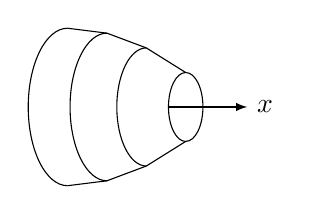
\begin{tikzpicture}[xscale=2,declare function={f(\x)=1-\x^2;}]
\pgfmathsetmacro{\a}{0}
\pgfmathsetmacro{\b}{0.75}
\pgfmathsetmacro{\c}{1/3*(\b-\a)}
\pgfmathsetmacro{\d}{2/3*(\b-\a)}
\pgfmathsetmacro{\ra}{f(\a)}
\pgfmathsetmacro{\rb}{f(\b)}
\pgfmathsetmacro{\rc}{f(\c)}
\pgfmathsetmacro{\rd}{f(\d)}
%\draw[gray]plot[domain=0:0.75]({\x},{f(\x)});
%\draw[gray]plot[domain=0:0.75]({\x},{-f(\x)});
\draw([shift={(90:1/4*\ra cm and \ra cm)}]\a,0) arc (90:270:1/4*\ra cm and \ra cm);
\draw([shift={(90:1/4*\rc cm and \rc cm)}]\c,0) arc (90:270:1/4*\rc cm and \rc cm);
\draw([shift={(90:1/4*\rd cm and \rd cm)}]\d,0) arc (90:270:1/4*\rd cm and \rd cm);
\draw(\b,0) circle (1/4*\rb cm and \rb cm);
\draw[-latex](\b-1/4*\rb,0)--++(0.5,0)node[right]{$x$};
\draw(\a,\ra)--(\c,\rc)--(\d,\rd)--(\b,\rb);
\draw(\a,-\ra)--(\c,-\rc)--(\d,-\rd)--(\b,-\rb);
\end{tikzpicture}
\caption{سطحی رقبہ مخروطی پٹیوں سے حاصل ہوتا ہے۔}
\end{subfigure}\hfill
\begin{subfigure}{0.45\textwidth}
\centering
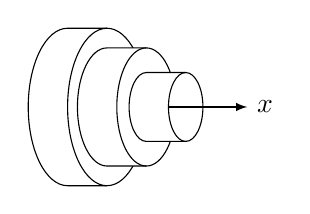
\begin{tikzpicture}[xscale=2,declare function={f(\x)=1-\x^2;}]
\pgfmathsetmacro{\a}{0}
\pgfmathsetmacro{\b}{0.75}
\pgfmathsetmacro{\c}{1/3*(\b-\a)}
\pgfmathsetmacro{\d}{2/3*(\b-\a)}
\pgfmathsetmacro{\len}{\d-\c}
\pgfmathsetmacro{\ra}{f(\a)}
\pgfmathsetmacro{\rb}{f(\b)}
\pgfmathsetmacro{\rc}{f(\c)}
\pgfmathsetmacro{\rd}{f(\d)}
%\draw[gray]plot[domain=0:0.75]({\x},{f(\x)});
%\draw[gray]plot[domain=0:0.75]({\x},{-f(\x)});
\draw[fill=white]([shift={(-90:1/4*\ra cm and \ra cm)}]\a,0) arc (-90:-270:1/4*\ra cm and \ra cm)--++(\len,0) arc (90:-90:1/4*\ra cm and \ra cm)--++(-\len,0);
\draw([shift={(90:1/4*\ra cm and \ra cm)}]\a+\len,0)arc (90:270:1/4*\ra cm and \ra cm);
\draw[fill=white]([shift={(-90:1/4*\rd cm and \rd cm)}]\c,0) arc (-90:-270:1/4*\rd cm and \rd cm)--++(\len,0) arc (90:-90:1/4*\rd cm and \rd cm)--++(-\len,0);
\draw([shift={(90:1/4*\rd cm and \rd cm)}]\d,0)arc (90:270:1/4*\rd cm and \rd cm);
\draw[fill=white]([shift={(-90:1/4*\rb cm and \rb cm)}]\d,0) arc (-90:-270:1/4*\rb cm and \rb cm)--++(\len,0) arc (90:-90:1/4*\rb cm and \rb cm)--++(-\len,0);
\draw([shift={(90:1/4*\rb cm and \rb cm)}]\d+\len,0)arc (90:270:1/4*\rb cm and \rb cm);
\draw[-latex](\b-1/4*\rb,0)--++(0.5,0)node[right]{$x$};
\end{tikzpicture}
\caption{سطحی رقبہ بیلنی پٹیوں سے حاصل نہیں ہوتا ہے۔}
\end{subfigure}
\caption{مخروط پٹی لینے سے کار آمد تکمل جبکہ بیلنی پٹی سے غیر کارآمد تکمل حاصل ہو گا۔}
\label{شکل_تکمل_استعمال_غلط_مثال}
\end{figure}

\جزوحصہء{مسئلہ پاپس}
وسطانی مراکز کا سطح طواف کے رقبہ اور جسم طواف کے حجم کے ساتھ تعلق کو \اصطلاح{مسئلہ پاپس}\فرہنگ{مسئلہ!پاپس}\حاشیہب{Pappus's theorem}\فرہنگ{Pappus's theorem} پیش کرتا ہے\حاشیہد{اسکندریا کا رہائشی قدیم یونانی ریاضی دان}۔

\ابتدا{مسئلہ}\موٹا{مسئلہ پاپس برائے حجم}
اگر کسی مستوی خطہ کو سطح مستوی میں لکیر کے گرد گھمایا جائے جہاں خطے کو لکیر قطع نہ کرتی ہو تب جسم طواف کا حجم خطے کا رقبہ ضرب وہ فاصلہ جو ایک چکر کے دوران وسطانی نقطہ طے کرتا ہو کے برابر ہو گا۔ اگر خطے کا رقبہ \عددی{S} اور وسطانی نقطے کا محور سے فاصلہ \عددی{\rho} ہو تب جسم طواف کا حجم درج ذیل ہو گا۔ 
\begin{align}
H=2\pi \rho S
\end{align}
\انتہا{مسئلہ}
%====================== 
\ابتدا{ثبوت}

\انتہا{ثبوت}
%=====================
